% hello.tex - Our first LaTeX example! This is a comment!

\documentclass{article}
\usepackage{graphicx}
%\usepackage{xunicode} % Unicode support for LaTeX character names (accents, European chars, etc)
\usepackage{xltxtra} % Extra customizations for XeLaTeX
\usepackage{color}
\usepackage{listings}
 

% "define" Scala
\lstdefinelanguage{Scala}{
  morekeywords={abstract,case,catch,class,def,%
    do,else,extends,false,final,finally,%
    for,if,implicit,import,match,mixin,%
    new,null,object,override,package,%
    private,protected,requires,return,sealed,%
    super,this,throw,trait,true,try,%
    type,val,var,while,with,yield},
  otherkeywords={=>,<-,<\%,<:,>:,\#,@},
  sensitive=true,
  morecomment=[l]{//},
  morecomment=[n]{/*}{*/},
  morestring=[b]",
  morestring=[b]',
  morestring=[b]"""
}


\definecolor{dkgreen}{rgb}{0,0.6,0}
\definecolor{gray}{rgb}{0.5,0.5,0.5}
\definecolor{mauve}{rgb}{0.58,0,0.82}

% Default settings for code listings
\lstset{frame=tb,
  language=Scala,
  aboveskip=3mm,
  belowskip=3mm,
  showstringspaces=false,
  columns=flexible,
  basicstyle={\small\ttfamily},
  numbers=none,
  numberstyle=\tiny\color{gray},
  keywordstyle=\color{blue},
  commentstyle=\color{dkgreen},
  stringstyle=\color{mauve},
  frame=single,
  breaklines=true,
  breakatwhitespace=true
  tabsize=3
}

\begin{document}
Hello world!

\textbf{bold!!!}

It does not matter whether you
enter one or several             spaces
after a word.

An empty line starts a new
paragraph.
\\ \\
\# \$ \% \~n \^o \~a

XeLaTeX: á,é,í

This is an % stupid
% Better: instructive <----
example: Supercal%
            ifragilist%
icexpialidocious

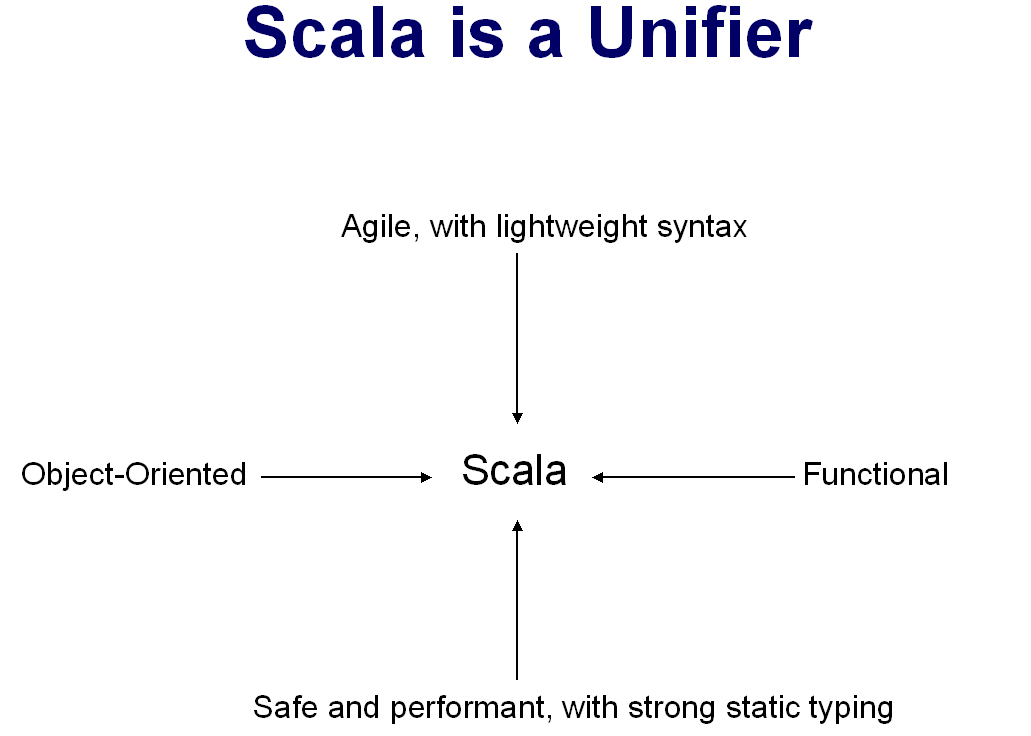
\includegraphics[scale=0.20]{Scala-is-a-Unifier.png}

    \begin{lstlisting}
    val t = "hello" 
    val x = 42 
    \end{lstlisting}

\end{document}